%%%%%%%%%%%%%%%%%%%%%%%%%%%%%%%%%%%%%%%%%
% Programming/Coding Assignment
% LaTeX Template
%
% This template has been downloaded from:
% http://www.latextemplates.com
%
% Original author:
% Ted Pavlic (http://www.tedpavlic.com)
%
% Note:
% The \lipsum[#] commands throughout this template generate dummy text
% to fill the template out. These commands should all be removed when 
% writing assignment content.
%
% This template uses a Perl script as an example snippet of code,
% most other languages are also usable. Configure them in the
% "CODE INCLUSION CONFIGURATION" section.
%%%%%%%%%%%%%%%%%%%%%%%%%%%%%%%%%%%%%%%%%

%-------------------------------------------------------------------------
%	PACKAGES AND OTHER DOCUMENT CONFIGURATIONS
%-------------------------------------------------------------------------

\documentclass{article}

\usepackage{fancyhdr} % Required for custom headers
\usepackage{lastpage} % Required to determine the last page for the footer
\usepackage{extramarks} % Required for headers and footers
\usepackage[usenames,dvipsnames]{color} % Required for custom colors
\usepackage{graphicx} % Required to insert images
\usepackage{listings} % Required for insertion of code
\usepackage{courier} % Required for the courier font
\usepackage{hyperref}
\usepackage{amsmath}
\usepackage{mathrsfs}
\usepackage{float}
\usepackage{enumitem}
\usepackage[english]{babel}
\usepackage[utf8]{inputenc}
\usepackage{fontenc}
\usepackage{booktabs}
\usepackage{pdfpages}
% Margins
\topmargin=-0.45in
\evensidemargin=0in
\oddsidemargin=0in
\textwidth=6.5in
\textheight=9.0in
\headsep=0.25in

\linespread{1.1} % Line spacing

% Set up the header and footer
\pagestyle{fancy}
\lhead{\hmwkAuthorName} % Top left header
\chead{\hmwkClassShort\ (\hmwkClassInstructor)} % Top center head
%\rhead{\firstxmark} % Top right header
\rhead{\hmwkTitle}
\lfoot{\lastxmark} % Bottom left footer
\cfoot{} % Bottom center footer
% Bottom right footer
\rfoot{Page\ \thepage\ of\ \protect\pageref{LastPage}} 
\renewcommand\headrulewidth{0.4pt} % Size of the header rule
\renewcommand\footrulewidth{0.4pt} % Size of the footer rule

\setlength\parindent{0pt} % Removes all indentation from paragraphs

%--------------------------------------------------------------------------
%	CODE INCLUSION CONFIGURATION
%--------------------------------------------------------------------------
% This is the color used for comments
\definecolor{MyDarkGreen}{rgb}{0.0,0.4,0.0} 
\lstloadlanguages{Perl,Python} % Load Perl syntax for listings,
% for a list of other languages supported see:
%ftp://ftp.tex.ac.uk/tex-archive/macros/latex/contrib/listings/listings.pdf
\lstset{language=Perl, % Use Perl in this example
        frame=single, % Single frame around code
        basicstyle=\small\ttfamily, % Use small true type font
        keywordstyle=[1]\color{Blue}\bf, % Perl functions bold and blue
        keywordstyle=[2]\color{Purple}, % Perl function arguments purple
        % Custom functions underlined and blue
        keywordstyle=[3]\color{Blue}\underbar, 
        identifierstyle=, % Nothing special about identifiers
        % Comments small dark green courier font
        commentstyle=\usefont{T1}{pcr}{m}{sl}\color{MyDarkGreen}\small, 
        stringstyle=\color{Purple}, % Strings are purple
        showstringspaces=false, % Don't put marks in string spaces
        tabsize=5, % 5 spaces per tab
        %
        % Put standard Perl functions not included
        % in the default language here
        morekeywords={rand},
        %
        % Put Perl function parameters here
        morekeywords=[2]{on, off, interp},
        %
        % Put user defined functions here
        morekeywords=[3]{test},
       	%
        % Line continuation (...) like blue comment
        morecomment=[l][\color{Blue}]{...}, 
        numbers=left, % Line numbers on left
        firstnumber=1, % Line numbers start with line 1
        numberstyle=\tiny\color{Blue}, % Line numbers are blue and small
        stepnumber=5 % Line numbers go in steps of 5
}


\lstset{language=Python, % Use Python in this example
        frame=single, % Single frame around code
        basicstyle=\small\ttfamily, % Use small true type font
        keywordstyle=[1]\color{Blue}\bf, % Python functions bold and blue
        keywordstyle=[2]\color{Purple}, % Python function arguments purple
        % Custom functions underlined and blue
        keywordstyle=[3]\color{Blue}\underbar, 
        identifierstyle=, % Nothing special about identifiers
        % Comments small dark green courier font
        commentstyle=\usefont{T1}{pcr}{m}{sl}\color{MyDarkGreen}\small, 
        stringstyle=\color{Purple}, % Strings are purple
        showstringspaces=false, % Don't put marks in string spaces
        tabsize=3, % 5 spaces per tab
        %
        % Put standard Python functions not included in the
        % default language here
        morekeywords={rand},
        %
        % Put Python function parameters here
        morekeywords=[2]{on, off, interp},
        %
        % Put user defined functions here
        morekeywords=[3]{test},
       	%
        % Line continuation (...) like blue comment
        morecomment=[l][\color{Blue}]{...}, 
        numbers=left, % Line numbers on left
        firstnumber=1, % Line numbers start with line 1
        numberstyle=\tiny\color{Blue}, % Line numbers are blue and small
        stepnumber=5 % Line numbers go in steps of 5
}


% Creates a new command to include a perl script, the first
% parameter is the filename of the script (without .pl), the
% second parameter is the caption
\newcommand{\perlscript}[2]{
\begin{itemize}
\item[]\lstinputlisting[caption=#2,label=#1]{#1.pl}
\end{itemize}
}
\newcommand{\pythonscript}[2]{
\begin{itemize}
\item[]\lstinputlisting[caption=#2,label=#1]{#1}
\end{itemize}
}
\newcommand{\tss}{\textsuperscript}
\newcommand{\tsbs}{\textsubscript}

%--------------------------------------------------------------------------
%	DOCUMENT STRUCTURE COMMANDS
%	Skip this unless you know what you're doing
%--------------------------------------------------------------------------

% Header and footer for when a page split occurs within a
% problem environment
\newcommand{\enterProblemHeader}[1]{
\nobreak\extramarks{#1}{#1 continued on next page\ldots}\nobreak
\nobreak\extramarks{#1 (continued)}{#1 continued on next page\ldots}\nobreak
}

% Header and footer for when a page split occurs between problem
% environments
\newcommand{\exitProblemHeader}[1]{
\nobreak\extramarks{#1 (continued)}{#1 continued on next page\ldots}\nobreak
\nobreak\extramarks{#1}{}\nobreak
}

\setcounter{secnumdepth}{0} % Removes default section numbers
% Creates a counter to keep track of the number of problems
\newcounter{homeworkProblemCounter} 

\newcommand{\homeworkProblemName}{}
\newenvironment{homeworkProblem}[1][Problem \arabic{homeworkProblemCounter}]{ % Makes a new environment called homeworkProblem which takes
   % 1 argument (custom name) but the default is "Problem #"
  % Increase counter for number of problems
  \stepcounter{homeworkProblemCounter}
  % Assign \homeworkProblemName the name of the problem
  \renewcommand{\homeworkProblemName}{#1}
  % Make a section in the document with the custom problem count
  \section{\homeworkProblemName}
  % Header and footer within the environment  
  \enterProblemHeader{\homeworkProblemName} 
}{
  % Header and footer after the environment
  \exitProblemHeader{\homeworkProblemName}
}
% Defines the problem answer command with the content as the only argument
 % Makes the box around the problem answer and puts the content inside
\newcommand{\problemAnswer}[1]{ 
\noindent\framebox[\columnwidth][c]{\begin{minipage}{0.98\columnwidth}#1\end{minipage}}
}

\newcommand{\homeworkSectionName}{}
\newenvironment{homeworkSection}[1]{ % New environment for sections within homework problems, takes 1 argument - the name of the section
\renewcommand{\homeworkSectionName}{#1} % Assign \homeworkSectionName to the name of the section from the environment argument
\subsection{\homeworkSectionName} % Make a subsection with the custom name of the subsection
\enterProblemHeader{\homeworkProblemName\ [\homeworkSectionName]} % Header and footer within the environment
}{
\enterProblemHeader{\homeworkProblemName} % Header and footer after the environment
}

% define ``struts'', as suggested by Claudio Beccari in
%    a piece in TeX and TUG News, Vol. 2, 1993.
\newcommand\Tstrut{\rule{0pt}{2.6ex}}         % = `top' strut
\newcommand\Bstrut{\rule[-0.9ex]{0pt}{0pt}}   % = `bottom' strut 
%--------------------------------------------------------------------------
%	NAME AND CLASS SECTION
%--------------------------------------------------------------------------
\newcommand{\hmwkTitle}{Homework\ 3} % Assignment title
\newcommand{\hmwkDueDate}{Saturday,\ December\ 10,\ 2016} % Due date
\newcommand{\hmwkClass}{NUEN 647\\ Uncertainty Quantification for Nuclear Engineering} % Course/class
\newcommand{\hmwkClassTime}{Tu/Th 11:10am} % Class/lecture time
\newcommand{\hmwkClassInstructor}{Dr. McClarren} % Teacher/lecturer
\newcommand{\hmwkAuthorName}{Paul Mendoza} % Your name
\newcommand{\hmwkClassShort}{NUEN 647 UQ for Nuclear Engineering}
%--------------------------------------------------------------------------
%	TITLE PAGE
%--------------------------------------------------------------------------

\title{
\vspace{2in}
\textmd{\textbf{\hmwkClass\ \hmwkTitle}}\\
\normalsize\vspace{0.1in}\small{Due\ on\ \hmwkDueDate}\\
\vspace{0.1in}\large{\textit{\hmwkClassInstructor}}
\vspace{3in}
}

\author{\textbf{\hmwkAuthorName}}
\date{} % Insert date here if you want it to appear below your name

%--------------------------------------------------------------------------

\begin{document}

\maketitle

%--------------------------------------------------------------------------
%	TABLE OF CONTENTS
%--------------------------------------------------------------------------

%\setcounter{tocdepth}{1} % Uncomment this line if you don't want subsections listed in the ToC

\newpage
\tableofcontents
\newpage

%--------------------------------------------------------------------------
%	PROBLEM 1
%--------------------------------------------------------------------------

% To have just one problem per page, simply put a \clearpage after each problem

\begin{homeworkProblem}

  Fit the data in Table \ref{tab:1} to a linear model using

  \begin{enumerate}[label=(\alph*)]
  \item{Least squares}
  \item{Ridge Regression}
  \item{Lasso Regression}
  \end{enumerate}

  \begin{table}[H]
    \begin{center}
      \caption{Data to fit linear model $y=a+bx_1+cx_2$}
      \label{tab:1}
        \begin{tabular}{l l l l}
          \toprule
           & $x_1$ & $x_2$ & y\Tstrut\Bstrut\\
          \hline
          1 & 0.99 & 0.98 & 6.42\Tstrut\\
          2 & -0.75 & -0.76 & 0.20 \\
          3 & -0.50 & -0.48 & 0.80 \\
          4 & -1.08 & -1.08 & -0.57 \\
          5 & 0.09 & 0.09 & 4.75 \\
          6 & -1.28 & -1.27 & -1.42 \\
          7 & -0.79 & -0.79 & 1.07 \\
          8 & -1.17 & -1.17 & 0.20 \\
          9 & -0.57 & -0.57 & 1.08 \\
          10 & -1.62 & -1.62 & -0.15 \\
          11 & 0.34 & 0.35 & 2.90 \\
          12 & 0.51 & 0.51 & 3.37 \\
          13 & -0.91 & -0.92 & 0.05\\
          14 & 1.85 & 1.86 & 5.50 \\
          15 & -1.12 & -1.12 & 0.17 \\
          16 & -0.70 & -0.70 & 1.72 \\
          17 & 1.19 & 1.18 & 3.97 \\
          18 & 1.24 & 1.23 & 6.38 \\
          19 & -0.52 & -0.52 & 3.29 \\
          20 & -1.41 & -1.41 & -1.49 \\
          \bottomrule
      \end{tabular}
    \end{center}
  \end{table}
  
  Be sure to do cross-validation for each fit, and for each method
  present your best estimate of the model.\\~\\
  \problemAnswer{
  Did this problem in R, and appended the PDF on the following
  pages.}
  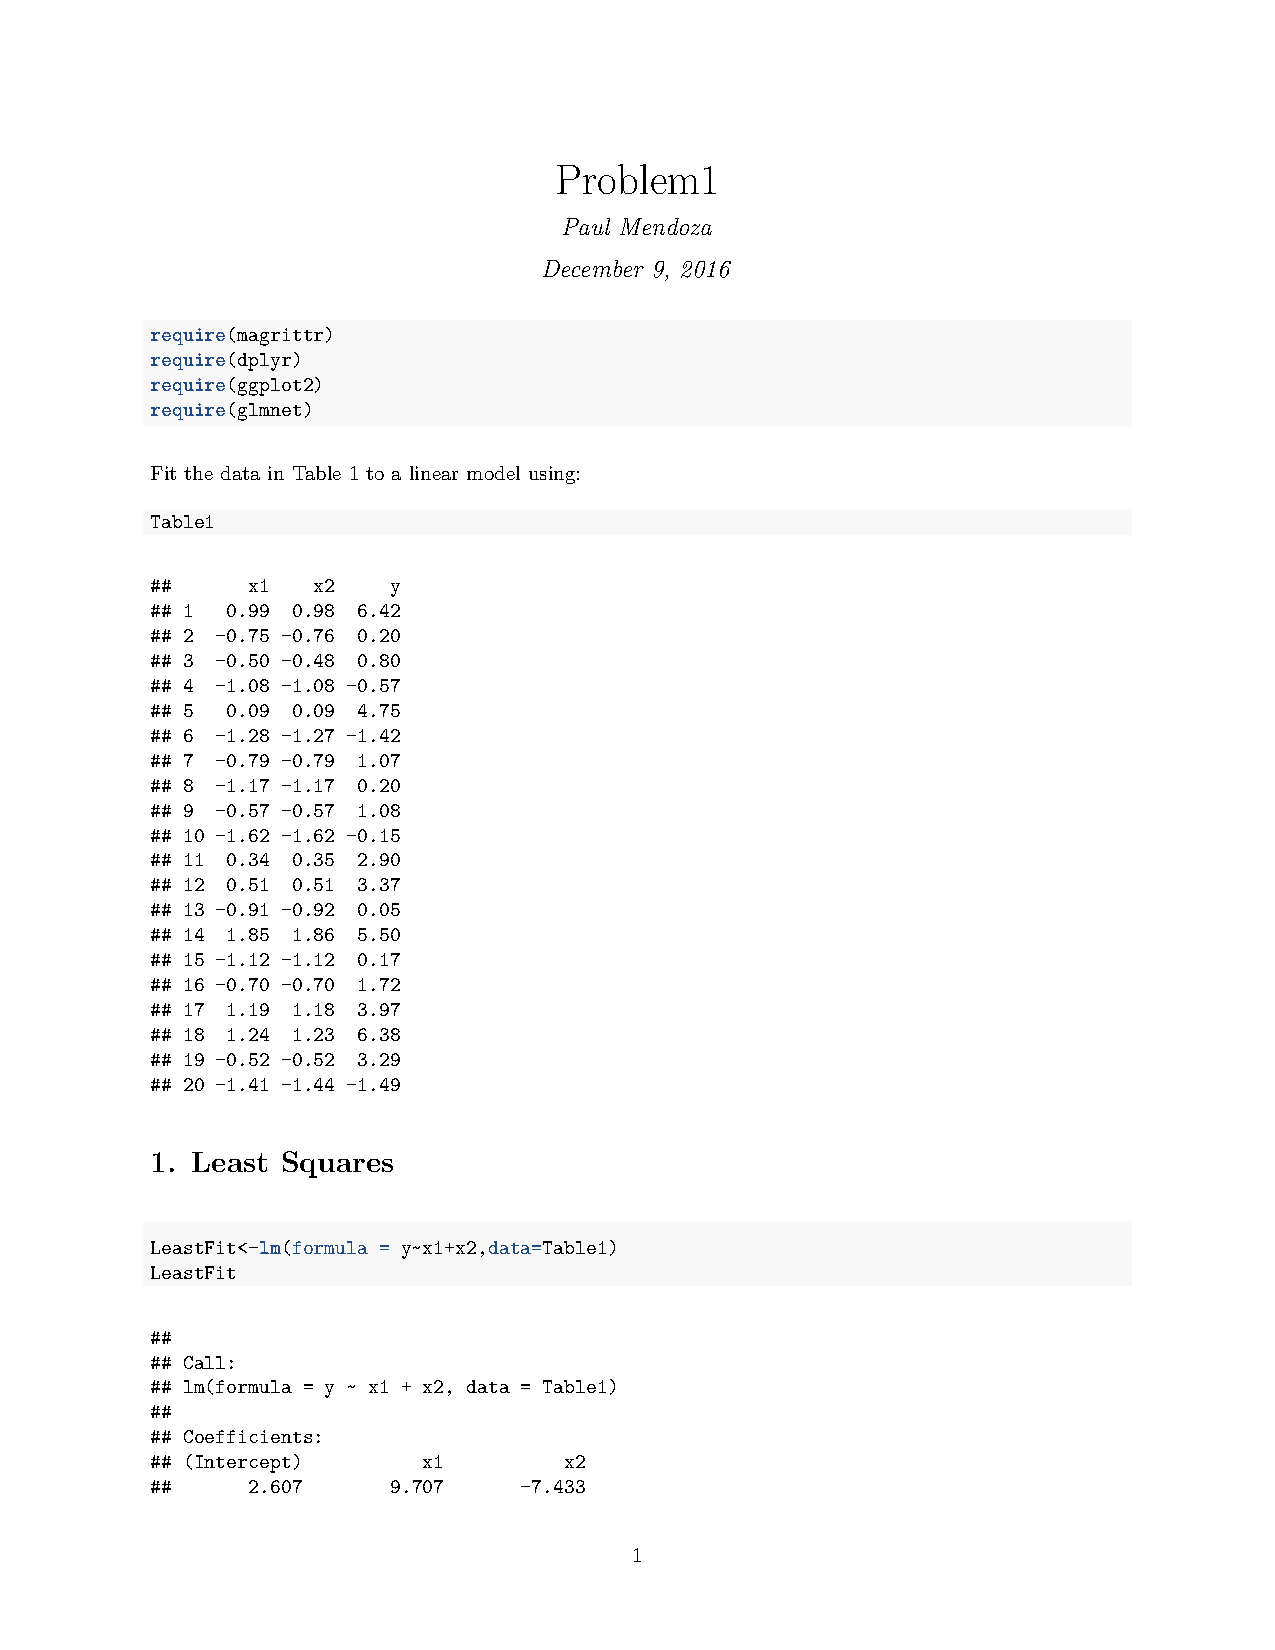
\includepdf[pages={1-10}]{Problem1_R/Problem1.pdf}
\end{homeworkProblem}

\clearpage



%--------------------------------------------------------------------------
%	PROBLEM 2
%--------------------------------------------------------------------------

\begin{homeworkProblem}
  Derive the adjoint operator for the equation
  \begin{equation*}
    -\bigtriangledown^2\phi(x,y,z)+\frac{1}{L^2}\phi(x,y,z)=\frac{Q}{D}
  \end{equation*}
  \begin{equation*}
    \phi(0,y,z)=\phi(x,0,z)=\phi(x,y,0)=\phi(X,y,z)=\phi(x,Y,z)
     =\phi(x,y,Z)=C
  \end{equation*}
  Compute the sensitivity to the QOI:
  \begin{equation*}
    QoI=\int_0^Xdx\int_0^Ydy\int_0^Zdz\frac{D}{L^2}\phi(x,y,z)
  \end{equation*}
  for X,Y,Z,L,, and Q.\\~\\

  \problemAnswer{
    \textbf{Derive the adjoint operator}\\~\\
    Define the operator $\mathcal{L}$ as
    \begin{equation*}
      \mathcal{L}=\bigtriangledown^2+\frac{1}{L^2}
    \end{equation*}
    and the adjoint $\mathcal{L^{\dag}}$ as
    \begin{equation*}
      \mathcal{L^{\dag}}=\bigtriangledown^2+\frac{1}{L^2}
    \end{equation*}
      \begin{equation*}
        \phi^\dag(0,y,z)=\phi^\dag(x,0,z)=
        \phi^\dag(x,y,0)=\phi^\dag(X,y,z)=\phi^\dag(x,Y,z)
     =\phi^\dag(x,y,Z)=C
      \end{equation*}
      Setting:
      \begin{equation*}
        \left|\frac{\delta\phi^\dag}{\delta x}\right|_{x=0}
        =
        \left|\frac{\delta\phi}{\delta x}\right|_{x=0}
      \end{equation*}
      and
      \begin{equation*}
        \left|\frac{\delta\phi^\dag}{\delta x}\right|_{x=X}
        =
        \left|\frac{\delta\phi}{\delta x}\right|_{x=X}
      \end{equation*}
      and similar for the other two dimentions.
    Also define the inner product as:
    \begin{equation*}
      (u,v)=\int_0^Xdx\int_0^Ydy\int_0^Zdz\ uv
    \end{equation*}
    
    \textit{Proof},
    in order to prove that this is an adjoint
    operator for the above equation, it needs to be shown that
    $(\mathcal{L}\phi,\phi^\dag)=(\phi,\mathcal{L}^\dag\phi^\dag)$.
    \\~\\
    Equivalent to:
    \begin{equation}
      \int_0^Xdx\int_0^Ydy\int_0^Zdz\left(\phi^\dag
      \bigtriangledown^2\phi+\phi^\dag\frac{\phi}{L^2}\right)
      =
      \int_0^Xdx\int_0^Ydy\int_0^Zdz\left(\phi\bigtriangledown^2\phi^\dag
      +\phi\frac{\phi^\dag}{L^2}\right)
    \end{equation}
    The terms
    \begin{equation*}
      \int_0^Xdx\int_0^Ydy\int_0^Zdz\left(\phi^\dag\frac{\phi}{L^2}\right)
      =
      \int_0^Xdx\int_0^Ydy\int_0^Zdz\left(\phi\frac{\phi^\dag}{L^2}\right)
    \end{equation*}
    are equal.
    For the other term with, $\bigtriangledown^2$, we can expand to:
    \begin{equation*}
      \int_0^Xdx\int_0^Ydy\int_0^Zdz\left(
      \phi^\dag\left[
        \frac{\delta^2\phi}{\delta x^2}+
        \frac{\delta^2\phi}{\delta y^2}+
        \frac{\delta^2\phi}{\delta z^2}
      \right]
      \right)
    \end{equation*}
  }
  \problemAnswer{
    Focusing on the $x$ terms, noting that $y$ and $z$
    will have the same derivation. Integration by parts,
    with $u=\phi^\dag$,
    $du=\frac{\delta\phi^\dag}{\delta x}dx$, and
    $v=\frac{\delta\phi}{dx}$,
    $dv=\frac{\delta^2\phi}{\delta x^2}dx$ yields.

    \begin{align*}
      \int_0^Ydy\int_0^Zdz\left(
      \int_0^Xdx\ \phi^\dag\frac{\delta^2\phi}{\delta x^2}
      \right)=
      \int_0^Ydy\int_0^Zdz\left(
      \left|
      \phi^\dag\frac{\delta\phi}{\delta x}
      \right|_{x=0}^{x=X}
      -\int_0^Xdx\ \frac{\delta\phi}{\delta x}
      \frac{\delta\phi^\dag}{\delta x}dx
      \right)
    \end{align*}
  
  Performing another integration by parts,
  with $u=\frac{\delta\phi^\dag}{\delta x}$,
  $du=\frac{\delta^2\phi^dag}{\delta x} dx$ and,
  $v=\phi$, $dv=\frac{\delta \phi}{\delta x} dx$.
  \begin{align*}
      =\int_0^Ydy\int_0^Zdz\left(
      \left|
      \phi^\dag\frac{\delta\phi}{\delta x}
      \right|_{x=0}^{x=X}
      -\left|
      \phi\frac{\delta\phi^\dag}{\delta x}
      \right|_{x=0}^{x=X}
      +\int_0^Xdx\ \phi
      \frac{\delta^2\phi^\dag}{\delta x^2}dx
      \right)
  \end{align*}
  At the boundaries, both $\phi$ and $\phi^\dag$ are
  a constant, and the derivatives of both at the
  boundaries are equal, and therefore those terms cancel,
  leaving
  \begin{align*}
    \int_0^Ydy\int_0^Zdz\left(
      \int_0^Xdx\ \phi
      \frac{\delta^2\phi^\dag}{\delta x^2}dx
      \right)
  \end{align*}
  which is equal to the $x$ component of the $\bigtriangledown^2$
  term of the RHS of equation 1 above. 
  }


  \vspace{5mm}

  
  \problemAnswer{
    \textbf{Compute the sensitivity to the QoI:}\\~\\
    I don't know if this is the right way to go about this,
    but if you modify the first equation listed in this problem to:
    \begin{equation*}
      \phi=L^2\left[\frac{Q}{D}+\bigtriangledown^2\phi\right]
    \end{equation*}
    and use it as a substitution, then we get something like this,
    \begin{align*}
      \text{QoI}&=\int_0^Xdx\int_0^Ydy\int_0^Zdz\
      \frac{D}{L^2}\phi\\
      &=\int_0^Xdx\int_0^Ydy\int_0^Zdz\
      \frac{D}{L^2}\left(
      L^2\left[\frac{Q}{D}+\bigtriangledown^2\phi\right]
      \right)\\
      &=\int_0^Xdx\int_0^Ydy\int_0^Zdz\
      \left[Q+D\bigtriangledown^2\phi\right]\\
    \end{align*}
    If $Q$ and $D$ both are independent of space, then
    \begin{align*}
      \text{QoI}=QXYZ+D\left[
        \int_0^Ydy\int_0^Zdz\
        \left|\frac{\delta\phi}{\delta x}\right|_{x=0}^{x=X}+
        \int_0^Xdx\int_0^Zdz\
        \left|\frac{\delta\phi}{\delta y}\right|_{y=0}^{y=Y}+
        \int_0^Xdx\int_0^Zdz\
        \left|\frac{\delta\phi}{\delta z}\right|_{z=0}^{z=Z}
        \right]
    \end{align*}
    I'm not sure how the adjoint helps me though.
  }
\end{homeworkProblem}

\clearpage


%--------------------------------------------------------------------------
%	PROBLEM 3
%--------------------------------------------------------------------------

\begin{homeworkProblem}
  For the random variable X $\sim$ N(0,1) draw fifty samples
  and generate histograms using the following sampling
  techniques
  \begin{enumerate}[label=(\alph*)]
  \item{Simple random sampling}
  \item{Stratifid sampling}
  \item{A van der Corput sequence of base 2}
  \item{A van der Corput sequence of base 3}
  \end{enumerate}

  \problemAnswer{
    Simple random sampling samples U(0,1) and plugs this value
    into the inverse CDF. Stratified sampling separates U(0,1)
    into equal bins and samples ``Randomly'' in each bin.
    Van der Corput sequences divides an interval into a a
    number of equal subintervals.
    \\~\\
    For example, the ordinary van der Corput sequence in
    base 3 is given by 1/3, 2/3, 1/9, 4/9, 7/9, 2/9, 5/9, 8/9, 1/27.
  }

  \pythonscript{Problem3/Calculations}{Script for Problem}

  \begin{figure}[H]
    \begin{center}
      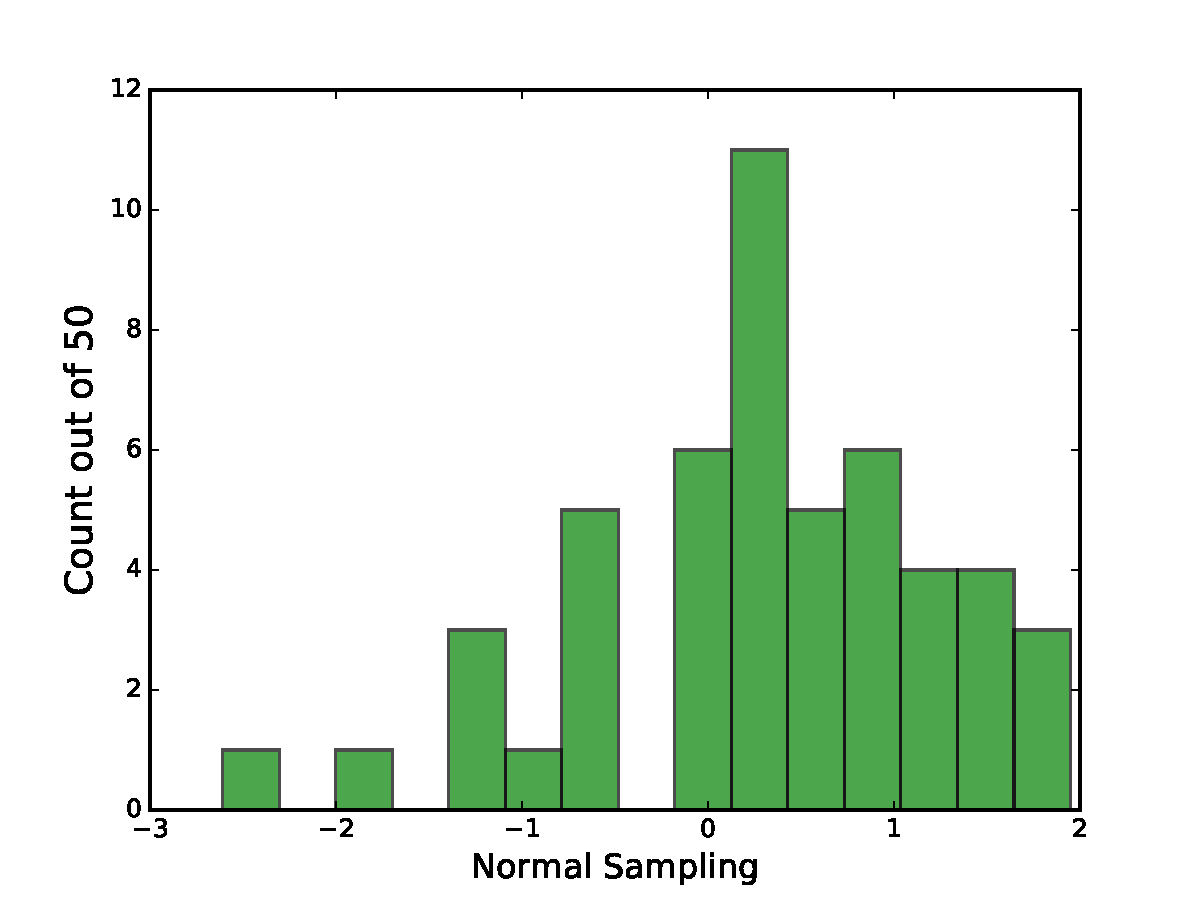
\includegraphics[width=0.77\columnwidth]{Problem3/NNorm.pdf}
    \end{center}
  \end{figure}

  \begin{figure}[H]
    \begin{center}
      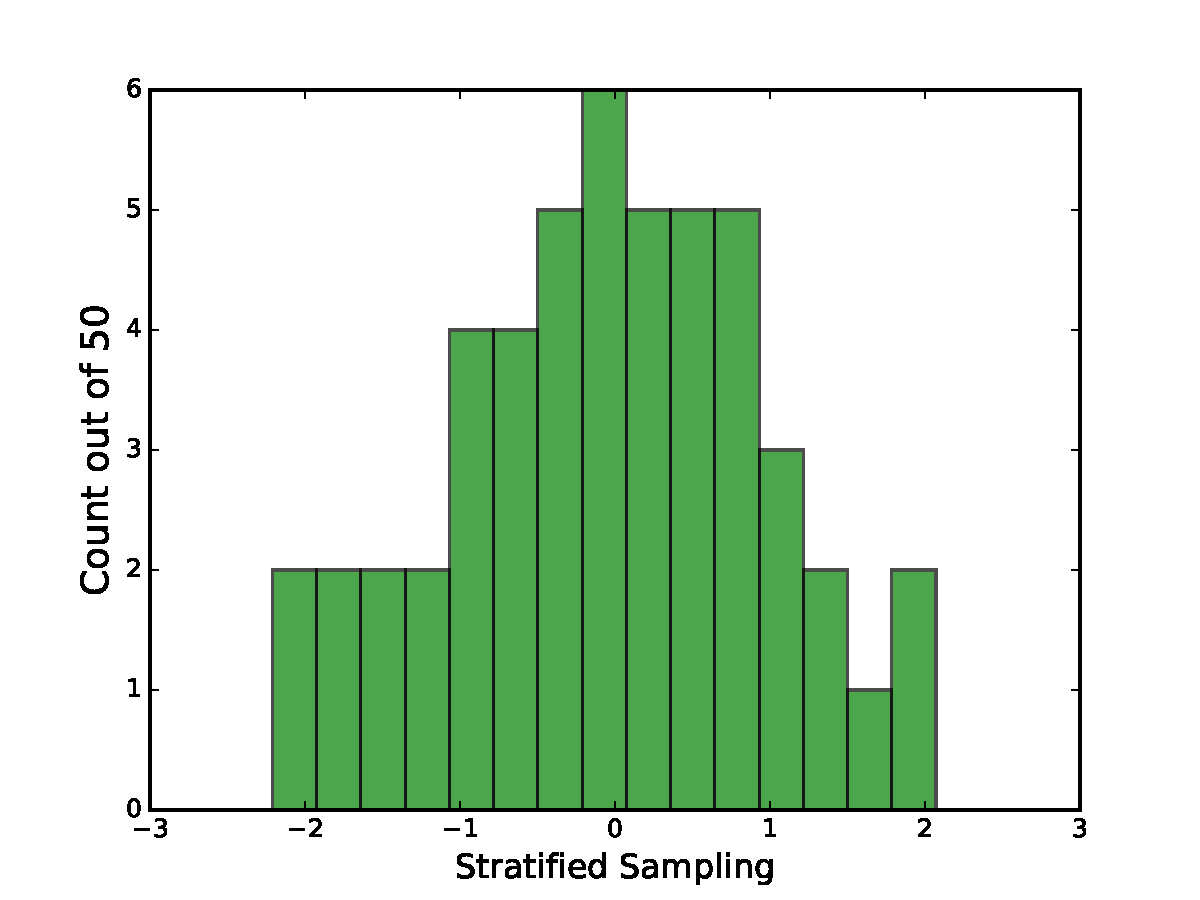
\includegraphics[width=0.77\columnwidth]{Problem3/SNorm.pdf}
    \end{center}
  \end{figure}

  \begin{figure}[H]
    \begin{center}
      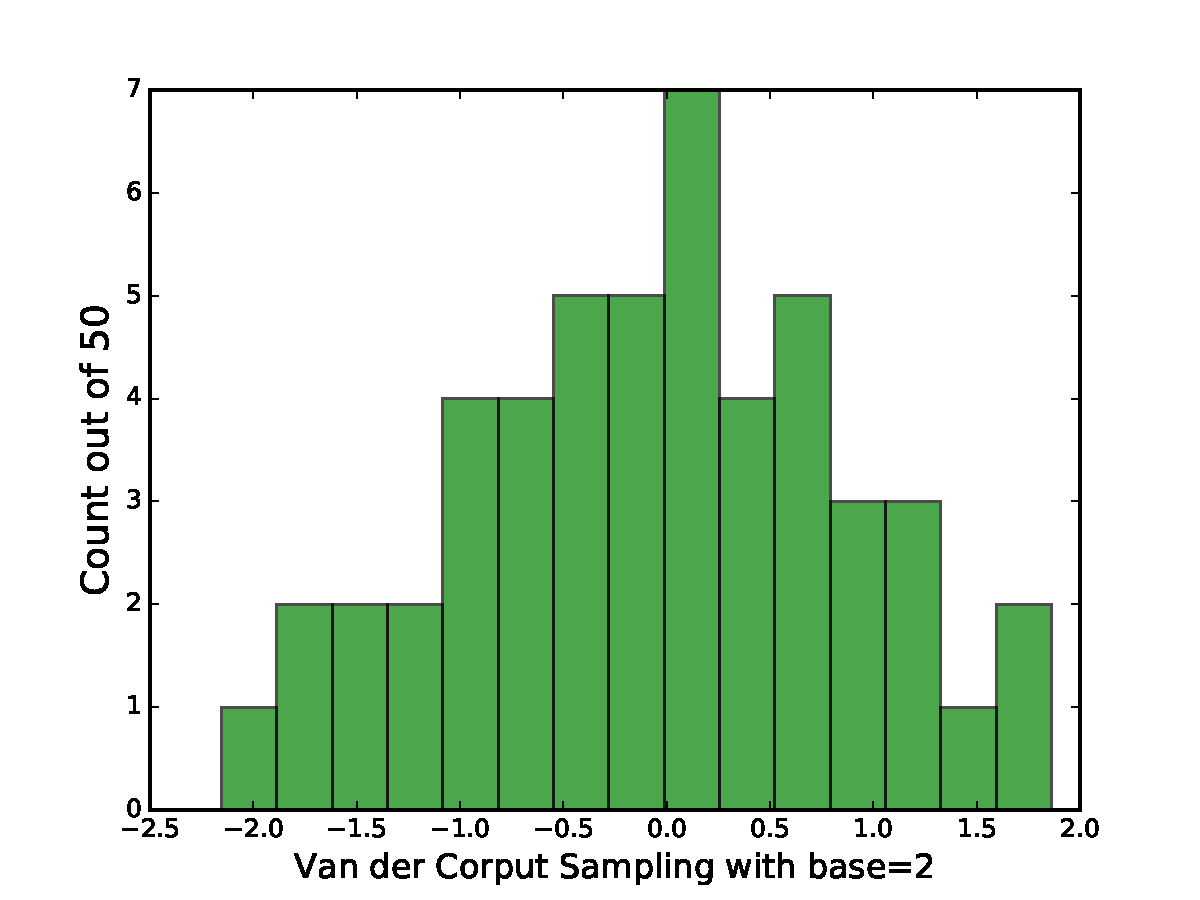
\includegraphics[width=0.77\columnwidth]{Problem3/V2Norm.pdf}
    \end{center}
  \end{figure}

  \begin{figure}[H]
    \begin{center}
      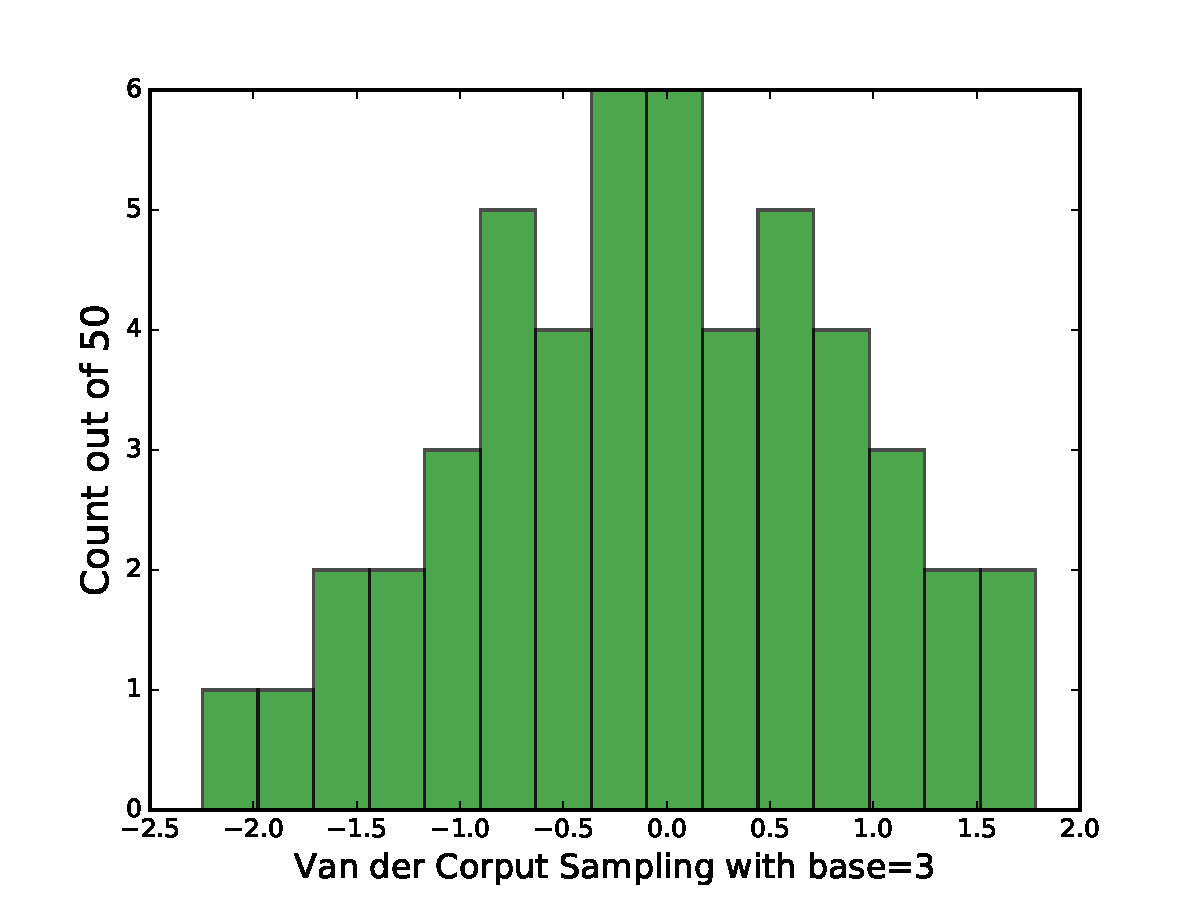
\includegraphics[width=0.77\columnwidth]{Problem3/V3Norm.pdf}
    \end{center}
  \end{figure}

\end{homeworkProblem}

\clearpage


%--------------------------------------------------------------------------
%	PROBLEM 4
%--------------------------------------------------------------------------

\begin{homeworkProblem}
  Consider the Rosenbrock function
  $f(x,y)=(1-x)^2+100(y-x^2)^2$. Assume that
  $x=2t-1$, where T $\sim\ B(3,2)$ and
  $y=2s-1$, where S $\sim\ B(1.1,2)$.
  Estimate the probability that $f(x,y)$ is
  less than 10 using:
  
  \begin{enumerate}[label=(\alph*)]
  \item{a first-order second-moment reliability method}
  \item{Latin hypercube sampling using 50 points}
  \item{A Halton sequence using 50 points}
  \end{enumerate}

  Compare this with the probability you calculate using
  10\tss{5} random samples. (\textit{Hint: Matlab has a
    built-in function for sampling beta R.V.'s ``betard''}).\\~\\
  
  \problemAnswer{
    The answer is simple
  }
  %\pythonscript{Problem4/Calculations}{Script for Problem}
\end{homeworkProblem}

\clearpage



%\pythonscript{Problem1/Calculations}{Script for Problem}
%% \begin{figure}[H]
%%   \begin{center}
%%     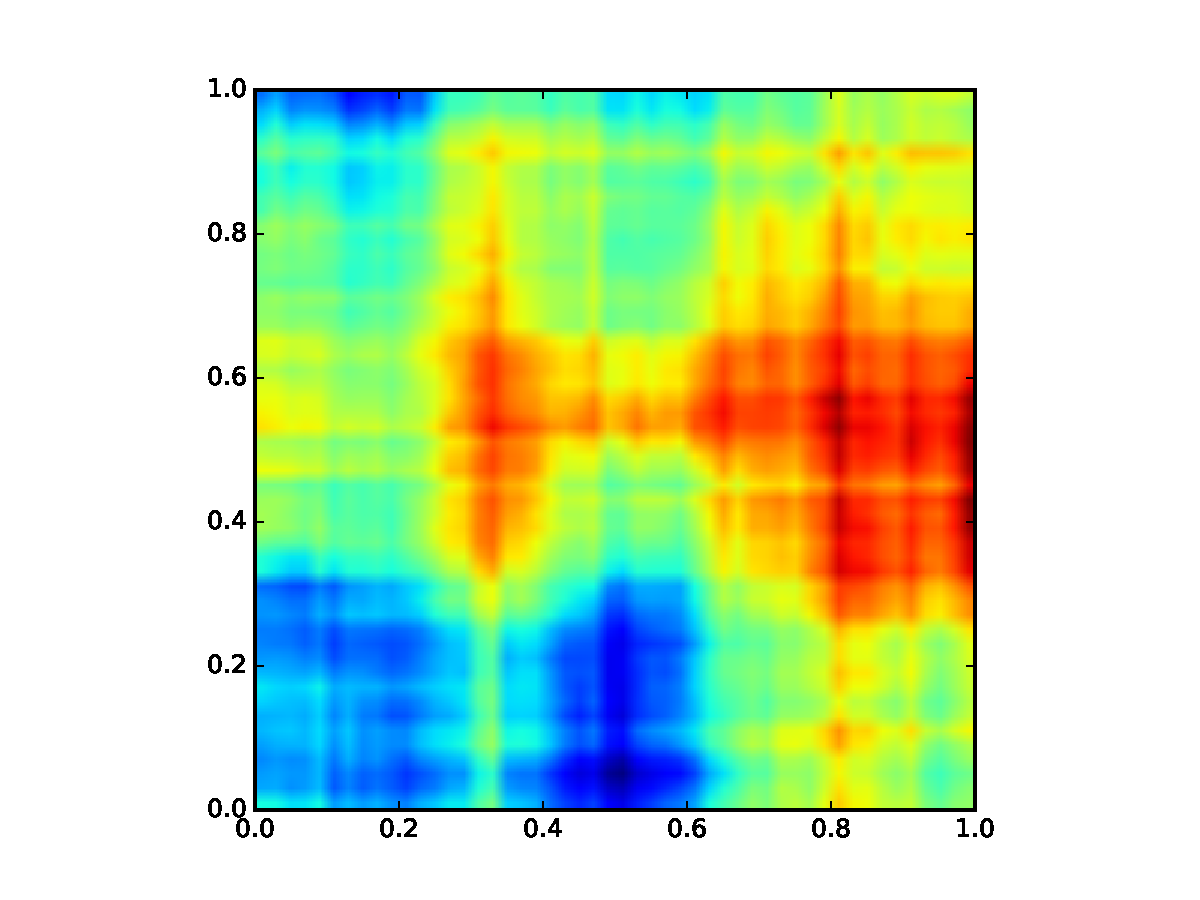
\includegraphics[width=0.77\columnwidth]{Problem1/P1realization1.pdf}
%%   \end{center}
%% \end{figure}
%\problemAnswer{TADA}

%--------------------------------------------------------------------------
%% This is an example citation \cite{Tatro2013}.
%% \bibliography{references} 
%% \bibliographystyle{plain} 

\end{document}
